\begin{frame}{\textbf{Fact 1:} there are persistent differences in \underline{the level} of the gender gap across CZ} 
\label{slide:fact1}
{\scriptsize\begin{center}
\begin{threeparttable}[!h]
\caption{CZ-level gender gap statistics}
\begin{tabular}{lcccccc}
\toprule
\toprule
& \multicolumn{6}{c}{\textbf{Census year}} \\
\cline{2-7}
\textbf{Statistic}&\multicolumn{1}{c}{\textbf{1970}}&\multicolumn{1}{c}{\textbf{1980}}&\multicolumn{1}{c}{\textbf{1990}}&\multicolumn{1}{c}{\textbf{2000}}&\multicolumn{1}{c}{\textbf{2010}}&\multicolumn{1}{c}{\textbf{2020}} \\
\midrule
Average gap         &        0.44         &        0.41         &        0.33         &        0.26         &        0.21         &        0.19         \\
Standard deviation  &        0.07         &        0.08         &        0.06         &        0.05         &        0.05         &        0.05         \\
\midrule\textbf{Distribution} \\
\midrule\hspace{0mm}p90&        0.53         &        0.51         &        0.40         &        0.32         &        0.26         &        0.25         \\
\hspace{0mm}p75     &        0.49         &        0.47         &        0.37         &        0.29         &        0.24         &        0.22         \\
\hspace{0mm}Median  &        0.44         &        0.41         &        0.33         &        0.26         &        0.21         &        0.19         \\
\hspace{0mm}p25     &        0.40         &        0.36         &        0.29         &        0.23         &        0.17         &        0.16         \\
\hspace{0mm}p10     &        0.35         &        0.32         &        0.26         &        0.20         &        0.15         &        0.13         \\
\bottomrule
\bottomrule
\end{tabular}
\end{threeparttable}
\end{center}
}
\textbf{\alert{Persistence:}} 20-year auto-correlation coefficient $>$ 50\%.

\beamerbutton{\hyperlink{slide:map}{Geographical pattern}}\hspace{1cm} \beamerbutton{\hyperlink{slide:map}{Persistence}}
\end{frame}

\begin{frame}{Fact 2: there is wide variation in the \underline{change} of gender wage gap across CZ}

\end{frame}
\begin{frame}{Fact 3: decline of the gender gap was faster in denser CZ}  				
	\begin{figure}[!h]
\centering
\caption{Change in male wage advantage in US CZ}
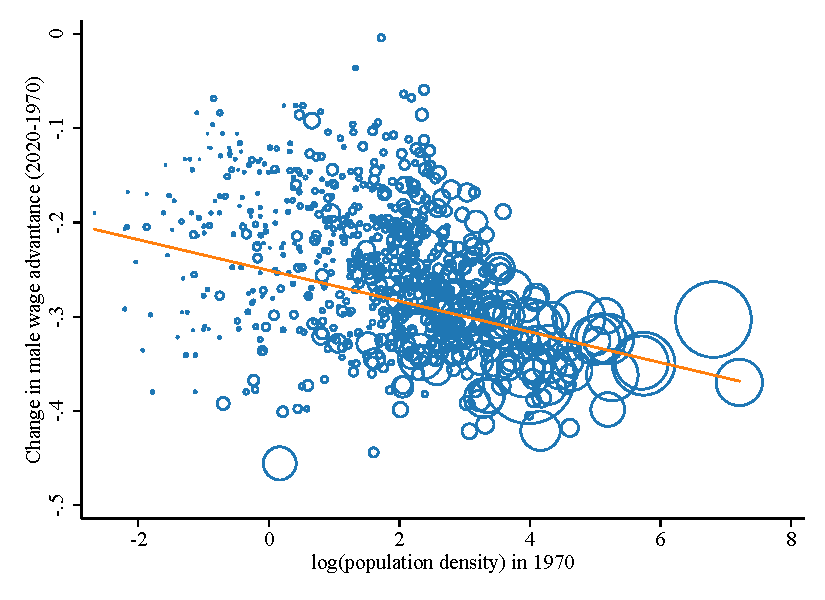
\includegraphics[width=.75\textwidth]{../2_analysis/output/figures/change_in_gap}
\end{figure}

\end{frame}
\begin{frame}{Fact 4: the gender gap - density gradient has \underline{inverted}}
	\label{slide:baseline}
	\textbf{\alert{Regression specification:}}	$w^{men}_{rt}-w^{women}_{rt}=\alpha_{rt}+\beta_{t}\ln(density)_{rt}+ \dots$
	\begin{figure}[!h]
\centering
\caption{Coefficient on population density $ \beta_t $}
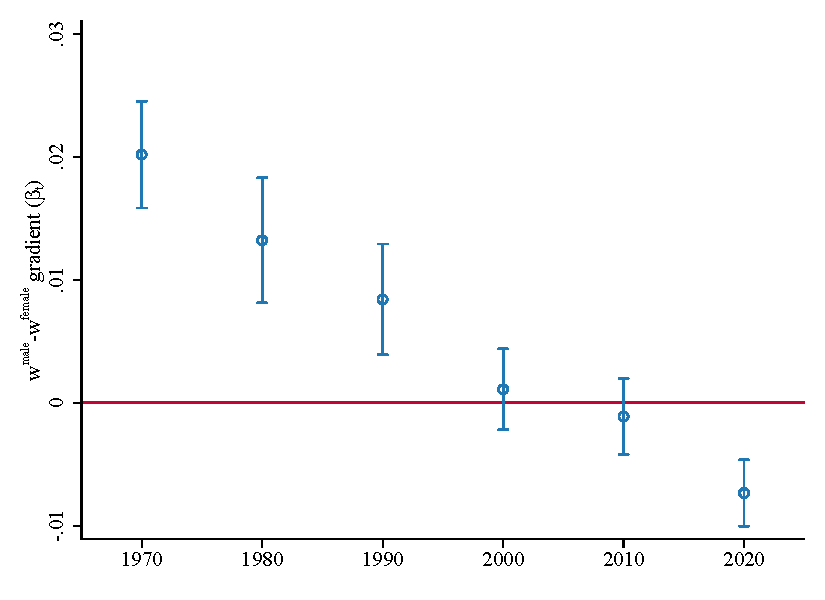
\includegraphics[width=.6\textwidth]{../2_analysis/output/figures/baseline_gradients_l_czone_density_full_time}
\par \begin{minipage}[h]{\textwidth}{\scriptsize\textbf{Note:} figure restricts to CZ with more than 1 people per km$^2$. Bars show 95\% robust confidence intervals.}\end{minipage}
\end{figure}

\beamerbutton{\hyperlink{slide:interpretation}{On coefficient size}} \hspace{.5cm} 	\beamerbutton{\hyperlink{slide:distribution}{Distribution illustration}}	 \hspace{.5cm} 	\beamerbutton{\hyperlink{slide:race}{Is this about gender?}} \hspace{.5cm}	\beamerbutton{\hyperlink{slide:married}{Within-group graphs}}		
\end{frame}

\begin{frame}{How big are these coefficients?}  
		\begin{center}
\begin{threeparttable}[!h]
\caption{Male advantange changes implied by estimated elasticities}
\label{tab:IC}
\begin{tabular}{lcccccc}
\toprule
\toprule
\textbf{}&\multicolumn{1}{c}{\textbf{1970}}&\multicolumn{1}{c}{\textbf{1980}}&\multicolumn{1}{c}{\textbf{1990}}&\multicolumn{1}{c}{\textbf{2000}}&\multicolumn{1}{c}{\textbf{2010}}&\multicolumn{1}{c}{\textbf{2020}} \\
\midrule
Density elasticity $ (\beta ) $&       0.020         &       0.013         &       0.008         &       0.001         &      -0.001         &      -0.007         \\
 \hspace{3mm} s.d. wage gap &       0.073         &       0.077         &       0.060         &       0.049         &       0.049         &       0.050         \\
$ \hspace{3mm}\beta / sd $&       0.278         &       0.173         &       0.141         &       0.022         &      -0.023         &      -0.146         \\
\midrule IC range   &       0.029         &       0.019         &       0.013         &       0.002         &      -0.002         &      -0.012         \\
\hspace{3mm} (\% mean gap) &       0.065         &       0.047         &       0.040         &       0.007         &      -0.009         &      -0.064         \\
 \midrule 90 - 10 pctile range  &       0.061         &       0.040         &       0.027         &       0.004         &      -0.004         &      -0.025         \\
\hspace{3mm} (\% mean gap)&       0.137         &       0.097         &       0.082         &       0.014         &      -0.018         &      -0.133         \\
\bottomrule
\bottomrule
\end{tabular}
\begin{tablenotes}
\item \footnotesize \textit{Note:} changes based on unweighted estimated elasticities. Sample restricted to full-time year-round workers. Table generated on 28 Sep 2020 at 15:15:18.
\end{tablenotes}
\end{threeparttable}
\end{center}

\end{frame}

\begin{frame}{What can account for the change in the density-gradient?}
	\label{slide:controls}
	\textbf{\alert{Regression specification:}} $w^{men}_{rt}-w^{women}_{rt}=\alpha_{rt}+\beta_{t}\ln(density)_t$
	\begin{figure}[!h]
\centering
\caption{Coefficient on population density $ \beta_t $ controlling for worker characteristics}
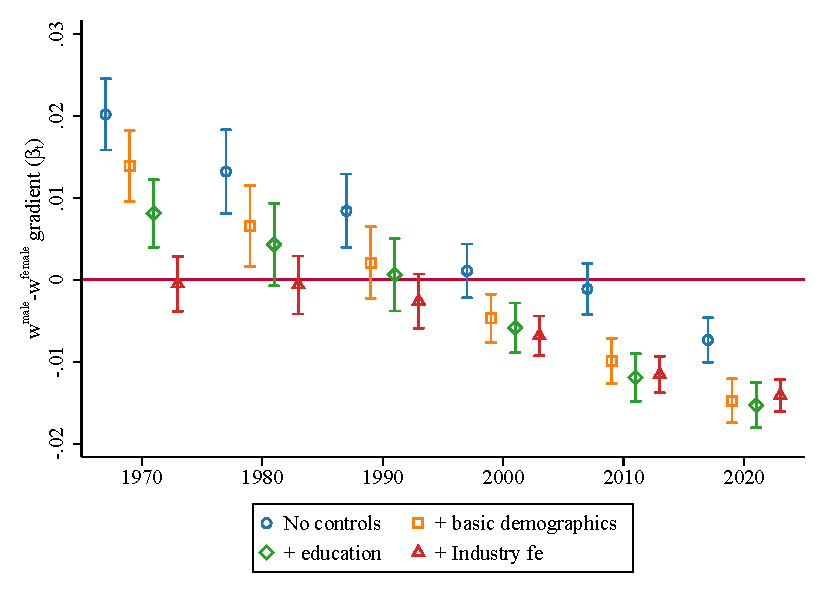
\includegraphics[width=.6\textwidth]{../2_analysis/output/figures/with_control_gradients_individual_l_czone_density_full_time}
\par \begin{minipage}[h]{\textwidth}{\tiny\textbf{Note:} figure restricts to CZ with more than 1 people per km$^2$. The regressions are done on data aggregated at the CZ level after residualizing individual-level characteristics. Bars show 95\% confidence intervals. Errors clustered at the CZ-level.}\end{minipage}
\end{figure}

	\beamerbutton{\hyperlink{slide:residual}{How do I control for individual characteristics?}}
\end{frame}

\begin{frame}{Adding czone-level variables}
	\label{slide:cz_controls}
	\textbf{\alert{Regression specification:}} $w^{men}_{rt}-w^{women}_{rt}=\alpha_{rt}+\beta_{t}\ln(density)_t+X_{rt}\gamma_t$
	\begin{figure}[!h]
\centering
\caption{Coefficient on population density $ \beta_t $ controlling for worker characteristics}
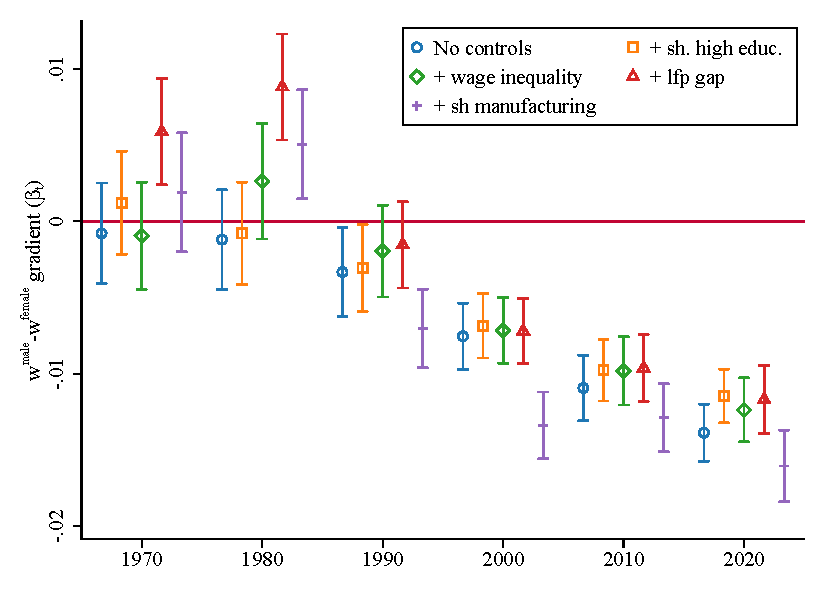
\includegraphics[width=.6\textwidth]{../2_analysis/output/figures/with_control_gradients_czone_l_czone_density_full_time}
\par \begin{minipage}[h]{\textwidth}{\tiny\textbf{Note:} figure restricts to CZ with more than 1 people per km$^2$. Regression includes census division $\times $ year fixed-effects. Additional controls include number of children, marital status and being a female head of household. The regressions are done on data aggregated at the CZ level. Bars show 95\% robust confidence intervals. Standard errors clustered at the CZ level. Figure generated on 19 Oct 2020 at 19:41:29. Figure generated using the dofile 2\_analysis/code\_files/write\_regression\_coefplots.do.}\end{minipage}
\end{figure}

	\beamerbutton{\hyperlink{slide:residual}{How do I control for individual characteristics?}}
\end{frame}